%%%%%%%%%%%%%%%%%%%%%%%%%%%%%%%
%%%%%%%%%%%%%%%%%%%%%%%%%%%%%%%
\chapter{Results\label{ch:results}}
%%%%%%%%%%%%%%%%%%%%%%%%%%%%%%%
This chapter presents a summary of the appended papers, including research activities
and a selection of the important results, and highlights the main achievements.

\section{Summary Paper \ref{pap:rolldamping}}
\subsection*{"\nameref{pap:rolldamping}"}
In Paper \ref{pap:rolldamping}, time series data from 250 roll decay tests (see Fig. \ref{fig:ship_types}) assembled from the Maritime Dynamics Laboratory at SSPA Sweden AB (\href{www.sspa.se}{www.sspa.se}) are used to investigate the roll motion model. 

\begin{figure}[H]
    \centering
    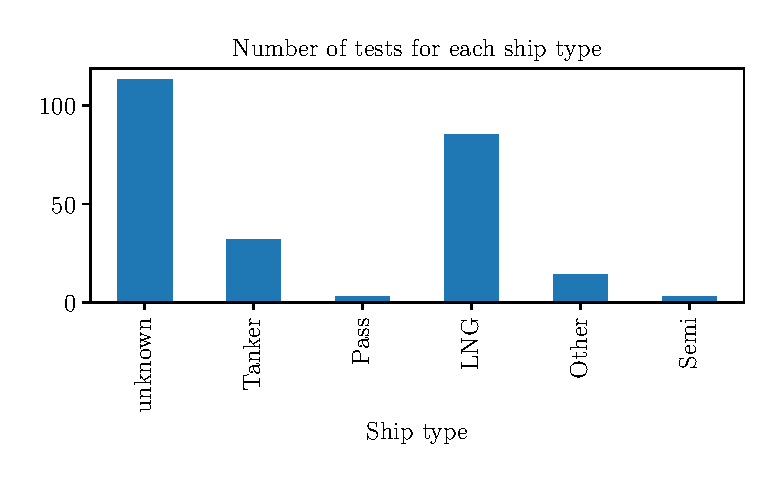
\includegraphics[width=0.5\columnwidth]{kappa/images/ship_types.eps}
    \caption{Number of tests per ship type}
    \label{fig:ship_types}
\end{figure}

\noindent Parameters in the linear (Eq.\ref{eq:roll_decay_equation_himeno_linear}), quadratic (Eq.\ref{eq:roll_decay_equation_himeno_quadratic_b}) and cubic (Eq.\ref{eq:roll_decay_equation_cubic}) roll motion model are identified using the roll motion PIT (see section \ref{sec:PIT_roll}). The quadratic damping model has almost the same accuracy as the cubic model and is therefore sufficient to reproduce most of the roll decay tests. The ''integration approach'' (see section \ref{sec:integration_approach}) to PIT roll motion, produces the most accurate models compared to the ''derivation approach'' (see section \ref{sec:derivation_approach}).

\subsection{Generic roll damping model}
\label{sec:genericrolldampingmodel}
A serial grey-box model for ship roll damping (see Fig.\ref{fig:greyrolldamping}) is developed in Paper \ref{pap:rolldamping}. 
This is expanding the system identification, not only focusing on one ship, but rather all modern ships, by a prediction model of the damping coefficients from the PIT applied on a whole database of roll decay tests. 
Simplified Ikeda's (SI) method \cite{kawahara_simple_2011} is used as the white box model, which is combined with a following black-box correction model.

\begin{figure}[H]
    
    \centering
    \begin{tikzpicture}[node distance=2cm]
    \node (white-box) [white-box] {Simplified Ikeda};
    \node (B_BK) [io, right of=white-box, xshift=0.90cm, yshift=1.5cm] {$\hat{B_{BK}}$};
    \node (B_E) [io, right of=white-box, xshift=0.75cm, yshift=0.75cm] {$\hat{B_{E}}$};
    \node (B_F) [io, right of=white-box, xshift=0.75cm, yshift=0cm] {$\hat{B_{F}}$};
    \node (B_L) [io, right of=white-box, xshift=0.75cm, yshift=-0.75cm] {$\hat{B_{L}}$};
    \node (B_W) [io, right of=white-box, xshift=0.75cm, yshift=-1.5cm] {$\hat{B_{W}}$};
    
    
    \node (black-box) [black-box, right of=B_F, xshift=0.75cm] {Black-box};
    \draw [arrow] (white-box) -- (B_BK);
    \draw [arrow] (white-box) -- (B_E);
    \draw [arrow] (white-box) -- (B_F);
    \draw [arrow] (white-box) -- (B_L);
    \draw [arrow] (white-box) -- (B_W);
    
    \draw [arrow] (B_BK) -- (black-box);
    \draw [arrow] (B_E)  -- (black-box);
    \draw [arrow] (B_F)  -- (black-box);
    \draw [arrow] (B_L)  -- (black-box);
    \draw [arrow] (B_W)  -- (black-box);
    
    
    \node (B) [io, right of=black-box, xshift=0.75cm, yshift=0cm] {$B$};
    \draw [arrow] (black-box)  -- (B);
    
    \end{tikzpicture}
    \caption{Grey-box model to predict roll damping}
    \label{fig:greyrolldamping}
\end{figure}

\noindent A roll damping dataset is used to train the black-box part of the grey-box model.
250 roll decay tests assembled from the Maritime Dynamics Laboratory at SSPA Sweden AB (\href{www.sspa.se}{www.sspa.se}) are used to build the dataset. The roll damping parameters are found by applying a PIT (see Section \ref{sec:PIT_roll}) on the parameterized roll motion models (see Section \ref{sec:roll}).
The black-box correction model of the output components from the SI method are shown in (Eq.\ref{eq:polynom_correction}),
\begin{equation} \label{eq:polynom_correction}
\hat{B_{e}} = 1.106 \hat{B_{BK}} - 0.9124 \hat{B_{E}} + 4.282 \hat{B_{F}} + 0.7457 \hat{B_{L}} + 0.1844 \hat{B_{W}} + 0.004999 \phi_{a} - 0.0005097
\end{equation}


\noindent Large corrections of the skin friction damping $\hat{B_F}$ and wave damping $\hat{B_W}$ are suggested by this expression. This is because the SI method is not very accurate for this dataset, where most of the ships in the dataset exceed the limits of the method. A pure black-box model is also devloped in Paper \ref{pap:rolldamping} (see Eq.\ref{eq:polynom_complex}),
\begin{equation} \label{eq:polynom_complex}
\begin{aligned} 
 \hat{B_{e}} = - 0.02578 A_{0} V - 0.02705 BK_{B} V + \\ 
 0.008993 BK_{L} V - 0.03191 C_{b} V - 0.2028 OG V + \\ 
 0.003472 V^{2} + \\ 
 0.004234 V \hat{\omega_{0}} - 0.002591 V \phi_{a} - 0.008384 V beam + \\ 
 0.05048 V + \\ 
 0.007814 \hat{\omega_{0}}^{2} + \\ 
 0.03882 \hat{\omega_{0}} \phi_{a} - 0.001069 \\ 
 \end{aligned}
\end{equation}


\noindent The grey-box model and the black-box model above, have about the same accuracy when performing cross-validation on the roll damping dataset.

\section{Summary Paper \ref{pap:daiyong}}
\subsection*{"\nameref{pap:daiyong}"}
Least Square Support Vector Regression (LS-SVR) \cite{brereton_support_2010} is used in Paper \ref{pap:daiyong} to identify the parameters in an Abkowitz Vessel Manoeuvring Model (AVMM) \cite{abkowitz_ship_1964}.  
The data is taken from experimental tests on a lake using a ship model with a scale of 50:1. The configuration of sensors and equipment for the experiment is shown in Fig.\ref{fig:cthmodel}.  
\begin{figure}[H]
    \centering
    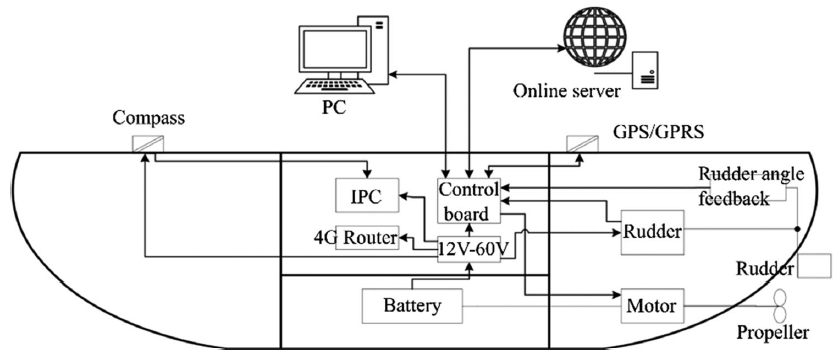
\includegraphics[width=\textwidth]{kappa/images/cth_model.png}
    \caption{Configuration of sensors and equipment for the experimental tests.}
    \label{fig:cthmodel}
\end{figure}
\noindent The hydrodynamic derivatives of the AVMM are identified almost perfectly when applied on data from simulations with MSS toolbox Mariner \cite{tristan_matlab_2009}. The PIT does however not work at all when applied on the data obtained from the lake experiments as seen in Fig.\ref{fig:daiyong_extrapolation}. 

\begin{figure}[H]
    \centering
    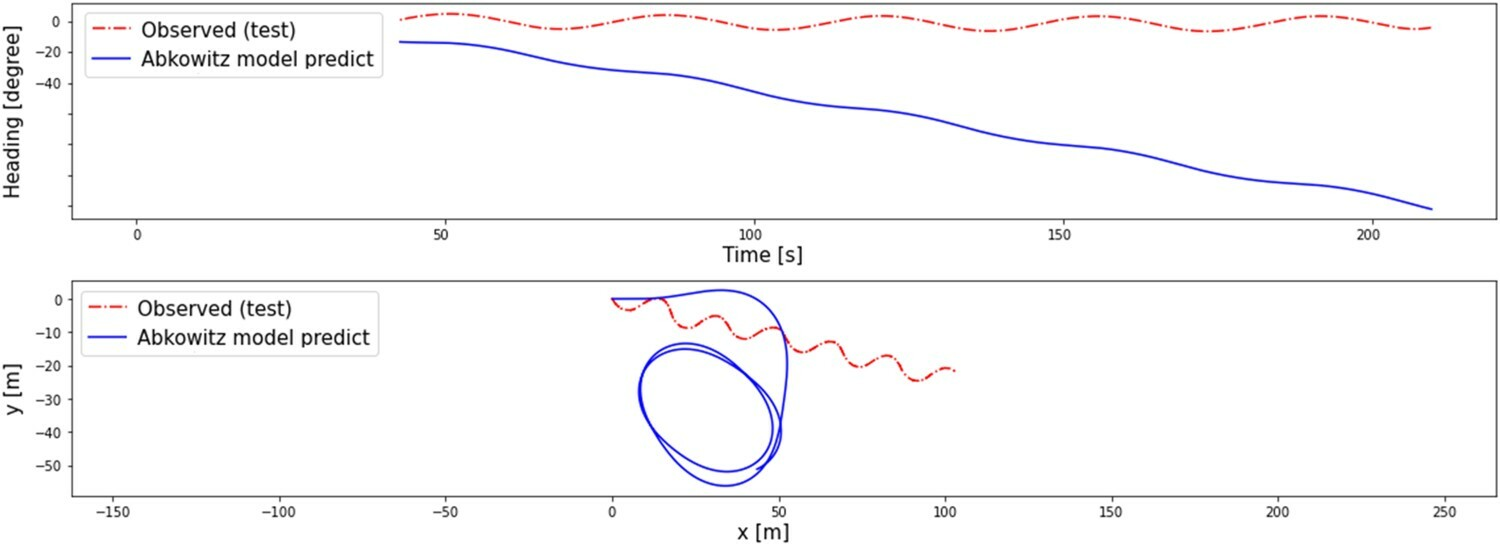
\includegraphics[width=\linewidth]{kappa/images/daiyong_extrapolation.jpeg}
    \caption{Prediction with AVMM of zigzag lake experiments.}
    \label{fig:daiyong_extrapolation}
\end{figure}

\noindent The PIT is very sensitive to noise due to the differentiation that needs to be conducted to calculate velocities and yaw rate from the measured position and heading. The PIT works better if the data is first cleaned using a proposed preprocessing algorithm together with a Kalman Filter (KF). The simulations with the identified model and the experiments are however still not in very good agreement.     

\section{Summary Paper \ref{pap:pit}}
\subsection*{"\nameref{pap:pit}"}
A method for System Identification of ship manoeuvring dynamics is developed in Paper \ref{pap:pit}. It is shown that the hydrodynamic derivatives within a VMM can be identified exactly at ideal conditions with no measurement noise and a perfect estimator.

It is shown that the proposed prepossessing of measurement data with EKF + RTS run in iteration with initial guess from semi-empirical formulas, is better than using low-pass filters for cleaning.

The new method can predict Turning circles with less than 5 \% error in advance and tactical diameter for the wPCC and KVLCC2 test cases, which should be considered sufficient considering the margin to the corresponding limits in the IMO standard for both ships.